\section{Multiple Linear Regression}
\textbf{\color{eblue}Example: } Consider the data:
  \begin{center}
    \begin{tabular}{|l|c|c|c|c|c|} 
         \hline
         $x$ & -1 & 1 & 2 & 3\\
         \hline 
         $y$ & 0.5 & -1 & -0.5 & 2\\
         \hline
    \end{tabular}
\end{center}
The the plot does not look linear:
\begin{center}
    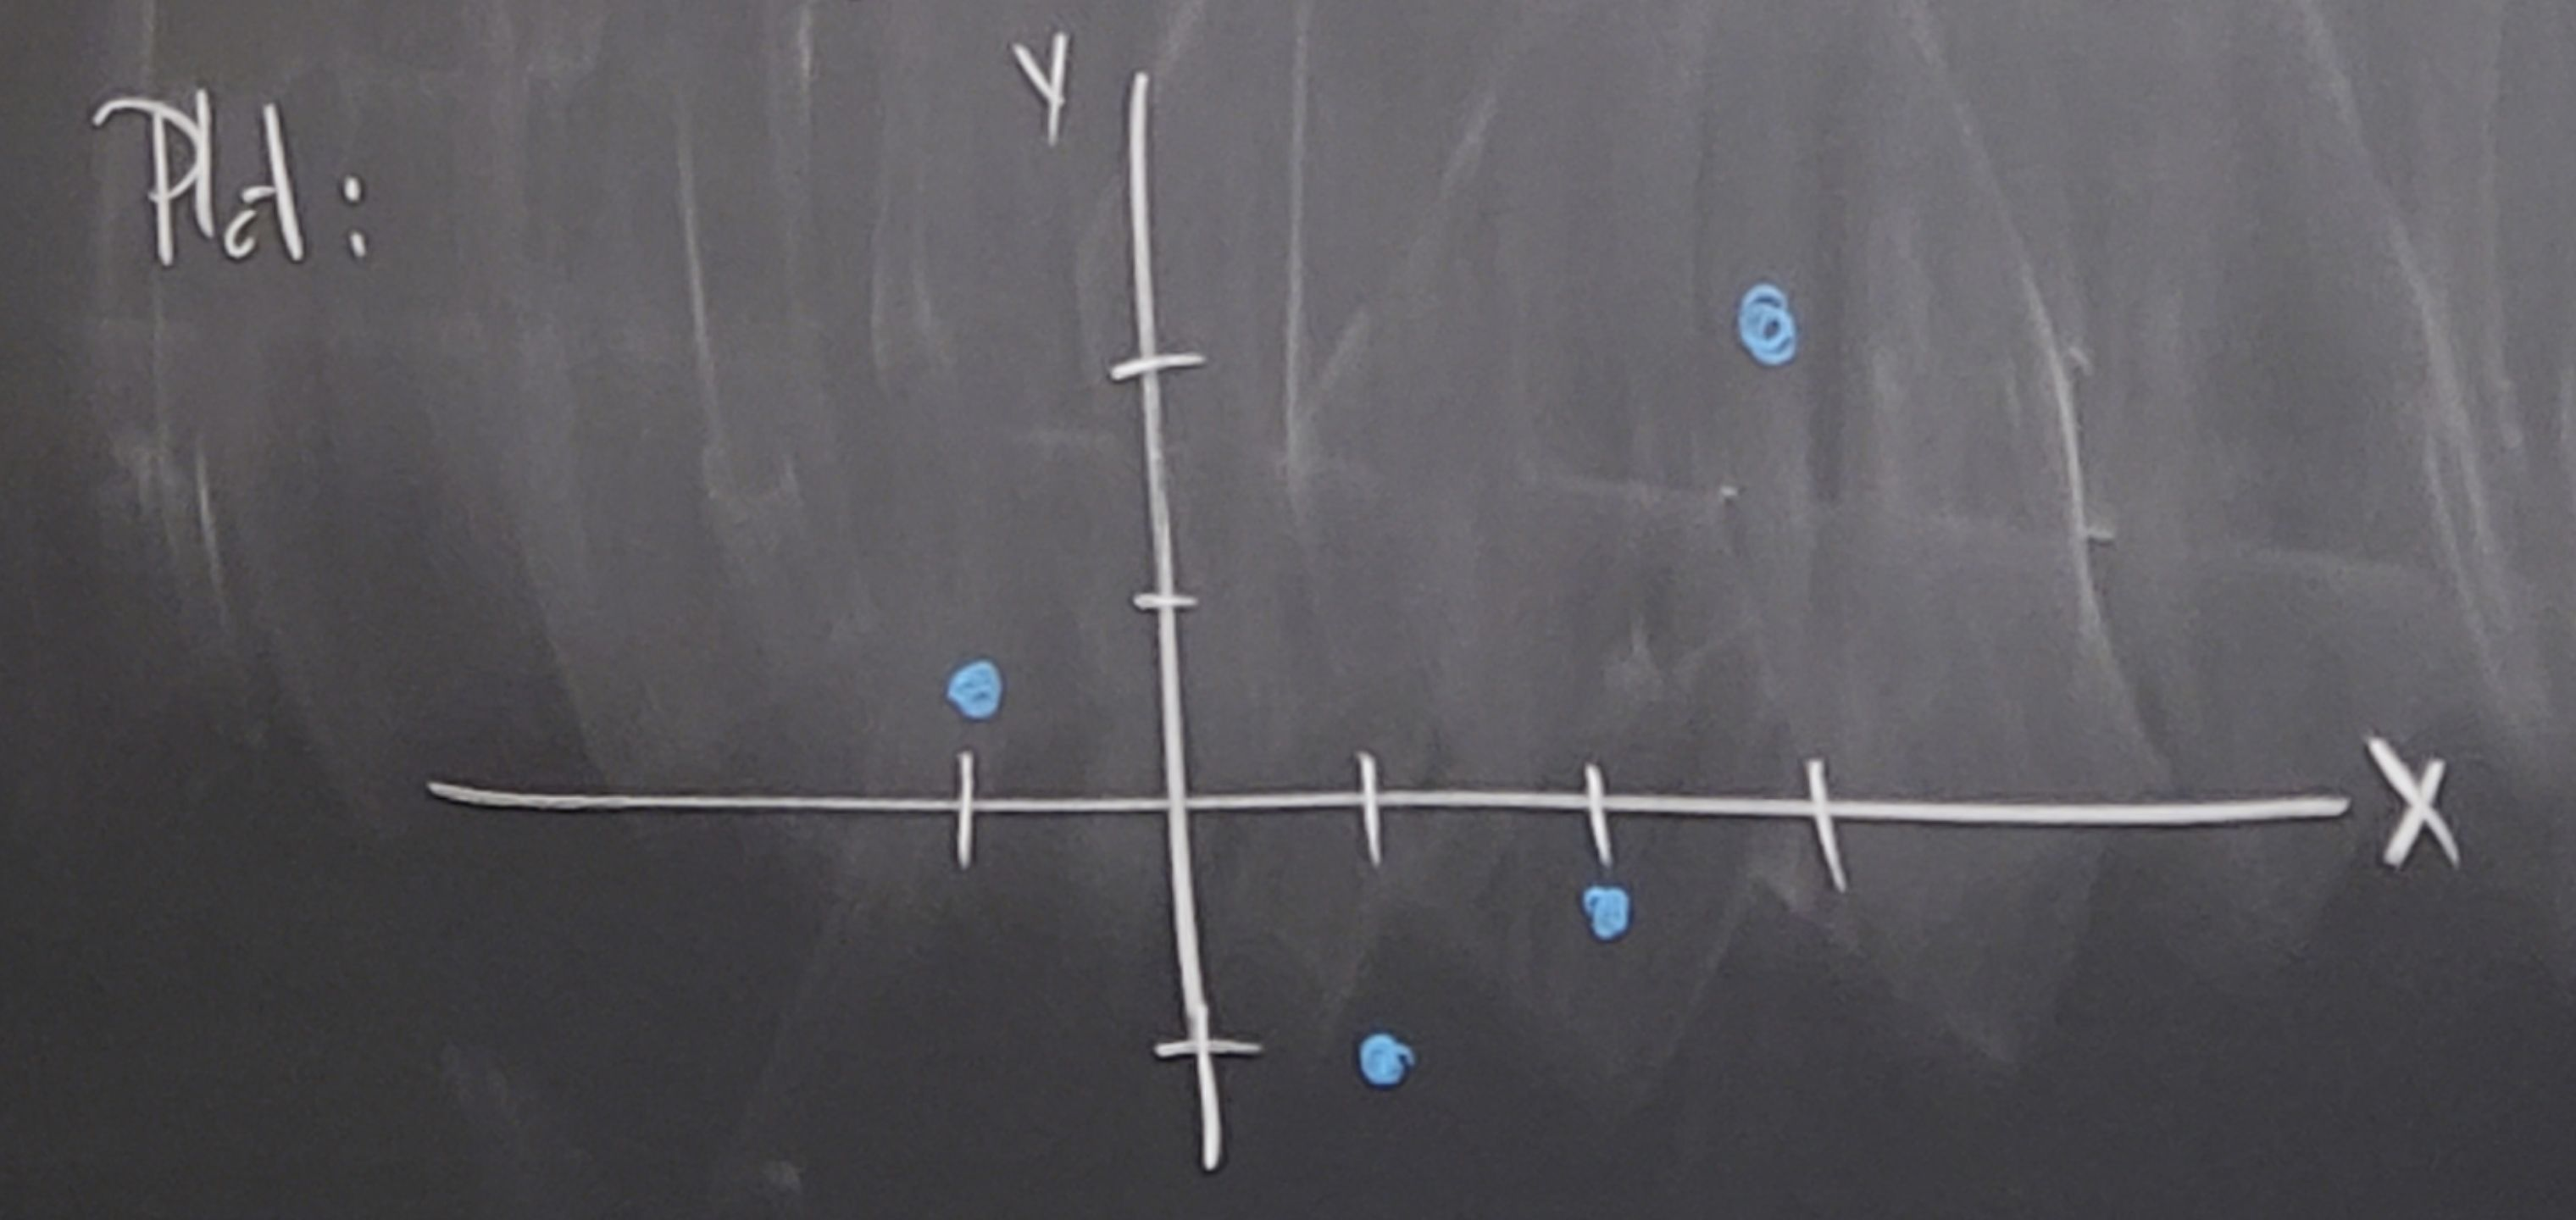
\includegraphics[height=2in]{11_10 plot.jpg}
\end{center}

\nl Seems unlikely that a line will fit well. What about a parabola? Want $y = \beta_0 + \beta_1x + \beta_2x^2$. Of course, in the probabilistic setup:
$$y = \underbrace{\beta_0 + \beta_1x + \beta_2x^2}_{\text{deterministic}} + \setRed \underbrace{ \varepsilon}_{\text{error}}$$
Using the data:
\begin{align*}
    \over{2} &= \beta_0 + \beta_1(-1) + \beta_2(-1)^2\\
    -1 &= \beta_0 + \beta_1(1) + \beta_2(1)^2 \\
    -\over{2} &= \beta_0 + \beta_1(2) + \beta_2(2)^2\\
    2 &= \beta_0 + \beta_1(3) + \beta_2(3)^2
\end{align*}
But this is the same idea as before, just in higher dimensions (3 coefficents).
$$\vec y = \beta_0 \vec 1 + \beta_1 \vec x + \beta_2 \vec{x^2}$$
$$= \beta_0 \begin{pmatrix}
    1\\1\\1\\1
\end{pmatrix} + \beta_1 \begin{pmatrix}
    -1\\1\\2\\3
\end{pmatrix} + \beta_2 \begin{pmatrix}
    1\\1\\4\\9
\end{pmatrix}$$
Or, as a matrix equation,
$$\begin{bmatrix}
    1 & -1 & 1\\ 1 & 1 & 1 \\ 1 & 2 & 4 \\ 1 & 3 & 9
\end{bmatrix} \begin{bmatrix}
    \beta_0 \\ \beta_1 \\ \beta_2
\end{bmatrix} = \begin{bmatrix}
    1/2 \\ -1 \\ -1/2 \\ 2
\end{bmatrix}.$$
Remark: This is why this process is called \textbf{linear} regression.

\nl The system for the coefficients will be a linear system. It has \red{nothing} to do with the underlying model\dots WHich here is quadratic $y = \beta_0 + \beta_1 x + \beta_2 x^2$.

\nl Just as before, we have an overdetermined system, which implies there is no solution. Hence, the best we can do is find the projection.

\nl We need a way to solve this projection problem in general. 

\nnl \textbf{Topic: The Normal Equations: }\\
In complete generality, $$y = \beta_0 + \beta_1 f_1(x) + \beta_2 f_2(x) + \cdots + \beta_n f_n(x) + \varepsilon.$$
Let there be $m$ data points $(x_i, y_i)$.

\nl This yields a matrix equation:
$$\begin{bmatrix}
    1 & f_1(x_1) & f_2(x_1) & \cdots & f_n(x_1)\\
    1 &  f_1(x_2) & f_2(x_2) & \cdots & f_n(x_2)\\
    \vdots & \vdots & \vdots & \ddots & \vdots \\
    1 &  f_1(x_n) & f_2(x_n) & \cdots & f_n(x_n)\\
\end{bmatrix} \begin{bmatrix}
    \beta_0 \\ \beta_1 \\ \vdots \\ \beta_n
\end{bmatrix} = \begin{bmatrix}
    y_1\\ y_2 \\ \vdots \\ y_n
\end{bmatrix}$$
Write $\mathbf X \vec{\beta} = \vec y$. Then $\mathbf X$ is $m$x$n$.

\nl Note, this setup really only makes sense when the system is overdetermined (more equations than unknowns). That is, more rows then columns in $\mathbf X$. i.e. $m > n$. We seek the coefficient vectors $\widehat{\beta} = [\thru{\widehat{\beta}}]$ such that $\norm{y - \mathbf X \widehat{\beta}}$ is minimized (LSR).

\nl In the gernal case, there are 2 new issues to content with:
\begin{enumerate}[label=\textcircled{\raisebox{-1pt}{\arabic*}}]
    \item no reason the column vectors of $\mathbf X$ are actually a basis for $\operatorname{Col} \mathbf X (might just be a spanning set)$.
    \item Certainly no reason columns are an orthogonal set. 
\end{enumerate}
The implication of $\textcircled{\raisebox{-1pt}{1}}$ is that a least squares solution $\widehat{\beta}$ need not be unique. As for $\textcircled{\raisebox{-1pt}{2}}$, ends we don't need this. By definition $\vec y - \mathbf X \widehat{\beta}$ is orthogonal to $\operatorname{Col}\mathbf X$.

\nl In other words, $\vec y - \mathbf X \widehat{\beta}$ must lie in the null space of $\mathbf X ^T$. (Recall $(\operatorname{Col} )^{\perp} = \operatorname{null}A^T$).

\nl Thus, $\mathbf X^T (y - \mathbf X \widehat{\beta}) = \vec 0$. 
$$\implies \underbrace{\mathbf X^T y}_{m \text{ vector}} - \underbrace{\mathbf X^T \mathbf X \widehat{\beta}}_{m \text{ vector}} = \underbrace{0}_{m}$$
$$\implies \mathbf X^T \mathbf X \widehat{\beta} = \mathbf X^T y$$
Definition: The normal equations:
$$\mathbf X^T \mathbf X \widehat{\beta} = \mathbf X^T y$$

\nl Facts:
\begin{enumerate}[label=\textcircled{\raisebox{-1pt}{\arabic*}}]
    \item $\mathbf X^T \mathbf X$ is an $n$x$n$ matrix.
    \item The normal equation is always a consistent system. That is, there is a solution to the least squares problem.
    \item If the columns of $\mathbf X$ are linearly independent, then $\mathbf X^T \mathbf X$ is an invertible square matrix and the unique solution to the least squares problem is
    $$\widehat{\beta} = \pars{\mathbf X^T \mathbf X}^{-1}\mathbf X^T y$$ 
\end{enumerate}

\example Our best fit parabola. 

$$\mathbf X = \begin{bmatrix}
    1 & -1 & 1\\ 1 & 1 & 1 \\ 1 & 2 & 4 \\ 1 & 3 & 9
\end{bmatrix}, \qquad \mathbf X^T = \begin{bmatrix}
    1 & 1 & 1 & 1\\ -1 & 1 & 2 & 3 \\ 1 & 1 & 4 & 9
\end{bmatrix}$$
$$\widehat{\beta} = [\widehat{\beta}_0, \widehat{\beta}_1, \widehat{\beta}_2], \quad y = \brac{ \over{2}, -1, -\over2, 2 }$$
$$\mathbf X^T \mathbf X = \begin{bmatrix}
    4 & 5 & 15\\ 5 & 15 & 35 \\ 15 & 35 & 99
\end{bmatrix}$$
Note that $\operatorname{det} (\mathbf X^T \mathbf X ) = 440 \neq 0$ so it is invertible. 
\begin{align*}
    \widehat{\beta} &= (\mathbf X^T \mathbf X )^{-1} \mathbf X^T y\\
    &= \begin{bmatrix}
        -41/44\\ -379/440 \\ 53/88
    \end{bmatrix}
\end{align*}
So, the best-fit parabola is 
\begin{align*}
    y &= -\frac{41}{44} - \frac{379}{440}x + \frac{53}{88}x^2\\
    &\approx -0.932 - 0.861x +0.602x^2
\end{align*}


\disc{Revisit the best-fit line}

\nl Given $n$ $(x_i,\, y_i)$'s, $y = \beta_0 + \beta_1 x + \varepsilon$. 
$$\implies \begin{bmatrix}
    \vec 1 & \bar x
\end{bmatrix} \widehat{\beta} = \vec y \wideand \widehat{\beta} = \begin{bmatrix}
    \widehat{\beta}_0\\ \widehat{\beta}_1
\end{bmatrix}$$
Here $\mathbf X = \begin{bmatrix}
    \vec 1 & \bar x
\end{bmatrix}$ is a $n\,\text{x}\,2$ matrix and $\mathbf X^T = \begin{bmatrix}
    1^T\\ x^T
\end{bmatrix}$ is $2\,\text{x}\,n$.

\nl Then
\begin{align*}
    \mathbf X^T \mathbf X &= \begin{bmatrix}
        1^T\\ x^T
    \end{bmatrix} \begin{bmatrix}
        \vec 1 & \bar x
    \end{bmatrix}\\
    &= \begin{bmatrix}
        1 \cdot 1 & 1 \cdot x\\ x \cdot 1 & x \cdot x \end{bmatrix}\\
        &= \begin{bmatrix}
            n & \sum x_i\\ \sum x_i & \sum {x_i}^2
        \end{bmatrix}
\end{align*}
Normal equation $X^TX \widehat{\beta} = X^T y$. Can we solve uniquely? 

\begin{align*}
    \det (X^TX) &= n \sum {x_i}^2 - \pars{\sum x_i}^2\\
    &= n \sum {x_i}^2 - n^2 \bar x^2\\
    &= n \pars{\sum {x_i}^2 - n \bar x}\\
    &= n S_{xx}\\
    &>0
\end{align*}
Therefore $X^TX$ is invertible! ($\det A \ne 0 \iff A^{-1}$ exists)

\nl So $\widehat{\beta} = (X^TX)^{-1}X^Ty$

\recall* $\displaystyle \begin{bmatrix}
    a & b \\ c & d
\end{bmatrix}^{-1} = \over*{\det A} \bigbrac{(\operatorname{tr}A)I - A} = \over{ad-bc} \begin{bmatrix}
    d & -b\\ -c & a
\end{bmatrix}$.

\nl So $$\displaystyle (X^TX)^{-1} = \over{nS_{xx}} \begin{bmatrix}
    \sum {x_i}^2 & - \sum x_i \\  - \sum x_i & n
\end{bmatrix} $$
and
$$X^T y = \begin{bmatrix}
    1^T \\ x^T
\end{bmatrix} y = \begin{bmatrix}
    1 \cdot y \\ x \cdot y
\end{bmatrix} = \begin{bmatrix}
    \sum y_i\\ \sum x_i y_i
\end{bmatrix}$$
Then
\begin{align*}
    \widehat{\beta} &= \over{nS_{xx}} \begin{bmatrix}
        \sum {x_i}^2 & - \sum x_i\\ -\sum x_i & n
    \end{bmatrix} \begin{bmatrix}
        \sum y_i \\ \sum x_i y_i
    \end{bmatrix}
    \\
    &= \over{n S_{xx}} \begin{bmatrix}
        (\sum {x_i}^2)(\sum y_i) - (\sum x_i)(\sum x_i y_i)\\
        -(\sum x_i)(\sum y_i) + n \sum x_i y_i
    \end{bmatrix}
\end{align*}
Same $\widehat{\beta}_0, \widehat{\beta}_1$ as earlier. But wait there's more\dots, Look at $(X^TX)^{-1}$:
\begin{align*}
    (X^TX)^{-1} &= \over{nS_{xx}} \begin{bmatrix}
        \sum {x_i}^2 & -n \bar x\\ -n \bar x & n
    \end{bmatrix}\\
    &= \begin{bmatrix}
        \dfrac{\sum {x_i}^2}{n S_{xx}} & -\dfrac{\bar x}{S_{xx}}\\ -\dfrac{\bar x}{S_{xx}} & \dfrac{1}{S_{xx}}
    \end{bmatrix}
\end{align*}
And
\begin{align*}
    \sigma^2 (X^TX)^{-1} &= \begin{bmatrix}
        \Var{\betah_0} & \Cov (\betah_0, \betah_1)
        \\ \Cov (\betah_0, \betah_1)  & \Var{\betah_1}
    \end{bmatrix}
\end{align*}
\textbf{FACT:} This always happens. $\sigma^2 (X^TX)^{-1}$ is the table of covariances:
$$\sigma^2 - a_{i\,j} = \Cov (\betah_i, \betah_j) \quad \text{where} \quad [a_{i\,j}] = (X^TX)^{-1}$$
Lastly,
$$S^2 = \frac{\operatorname{SSE}}{n-2} = \frac{\displaystyle \sum (y_i - \widehat{y}_i)^2}{n-2}$$
And \say{by some matrix algebra} (Wackerly),
$$\operatorname{SSE} = y^Ty - \betah^T \mathbf X^T y.$$

\example* (Antibiotic again)
\begin{center}
    \begin{tabular}{|l||c|c|c|c|c|c|c|c|c|c|c|c|} 
         \hline
         $x$ & 30 & 30 & 30 & 50 & 50 & 50 & 70 & 70 & 70 & 90 & 90 &90 \\
         \hline 
         $y$ & 38 & 43 & 29 & 32 & 26 & 33 & 19 & 24 & 23 & 14 & 19 & 21\\
         \hline
    \end{tabular}
\end{center}
$n = 12$ and $X^TX \displaystyle = \bmat{n}{\sum x_i}{\sum x_i}{\sum {x_i}^2} = \bmat{12}{720}{720}{\num{49200}}$. Then $\det (X^TX) = \num{72000}$. Then
$$(X^TX)^{-1} = \over{\num{72000}} \begin{bmatrix}
    \num{49200} & -700 \\ -700 & 12
\end{bmatrix}.$$
\setRed \textbf{Note:} \setBlack $\Var*{\betah_0} = \dfrac{41}{60}\sigma^2$, and $\Var*{\betah_1} = \dfrac{\sigma^2}{6000}$. 

\nl Then $X^Ty \displaystyle = \vvec*{\sum y_i}{\sum x_iy_i} = \vvec*{324}{\num{17540}}$ and $\betah = (X^TX)^{-1}X^Ty = \vvec*{46}{-19/60}$ (same as before). Hence 
$$\widehat{y} = 46 - \frac{19}{60}x$$
$$\operatorname{SSE} = y^Ty - \betah^T X^Ty = \frac{2961}{15}$$
$$\sigma^2 \approx \frac{\operatorname{SSE}}{n-2} = \frac{2971/15}{10} \approx 19.8067.$$